Find the frequency of oscillation for the Hartley circuit in Fig. \ref{fig:ee18btech11019_fig1}.  Also find the condition on $g_m$.
\begin{figure}[!ht]
	\begin{center}
		\resizebox{\columnwidth}{!}{\begin{circuitikz}

	\draw
	% Drawing a npn transistor
	(0,0) node[npn](npn1){} 
	% Making connections from transistor using relative coordinates
	% Labelling the transistor
	(npn1.B) --++(-1,0) --++(0,-3)--++(3,0)
	(npn1.C) --++(0,0.5) --++(0.75,0) to[R=R](0.75,-1.25) -- (0,-1.25)
	(npn1.E)--++(0,-1) to node[ground]{}(0,-1.25);
	\draw (0.75,1.25) --++(1.25,0) to[L=$L_1$](2,-1.25)--(0.75,-1.25)
	(2,-1.25) to[L=$L_2$](2,-3) -- (1,-3)
	(2,1.25) -- (3,1.25) to[C=C](3,-3)--(2,-3)
	
	;
\end{circuitikz}
}
	\end{center}
\caption{Hartley oscillator}
\label{fig:ee18btech11019_fig1}
\end{figure}
%Below is the figure, 
\begin{enumerate}[label=\arabic*.,ref=\theenumi]
%\begin{enumerate}[label=\thesection.\arabic*.,ref=\thesection.\theenumi]
\numberwithin{equation}{enumi}
\numberwithin{figure}{enumi}
\item Draw the small signal model for Fig. \ref{fig:ee18btech11019_fig1} and the block diagram for the equivalent control system.
\\
\solution See Figs. \ref{fig:ee18btech11019_fig2} and \ref{fig:ee18btech11019_fig3}.
%
\renewcommand{\thefigure}{\theenumi.\arabic{figure}}
\begin{figure}[!ht]
	\begin{center}
		\resizebox{\columnwidth}{!}{%%%%%%%%%%%%%%%%%%%%%%%%%%%%%%%%%%%%%%%%%%%%%%%%%%%%%%%%%%%%%%%%%%%%%%
%%                                                                  %%
%%  This is the header of a LaTeX2e file exported from Gnumeric.    %%
%%                                                                  %%
%%  This file can be compiled as it stands or included in another   %%
%%  LaTeX document. The table is based on the longtable package so  %%
%%  the longtable options (headers, footers...) can be set in the   %%
%%  preamble section below (see PRAMBLE).                           %%
%%                                                                  %%
%%  To include the file in another, the following two lines must be %%
%%  in the including file:                                          %%
%%        \def\inputGnumericTable{}                                 %%
%%  at the beginning of the file and:                               %%
%%        \input{name-of-this-file.tex}                             %%
%%  where the table is to be placed. Note also that the including   %%
%%  file must use the following packages for the table to be        %%
%%  rendered correctly:                                             %%
%%    \usepackage[latin1]{inputenc}                                 %%
%%    \usepackage{color}                                            %%
%%    \usepackage{array}                                            %%
%%    \usepackage{longtable}                                        %%
%%    \usepackage{calc}                                             %%
%%    \usepackage{multirow}                                         %%
%%    \usepackage{hhline}                                           %%
%%    \usepackage{ifthen}                                           %%
%%  optionally (for landscape tables embedded in another document): %%
%%    \usepackage{lscape}                                           %%
%%                                                                  %%
%%%%%%%%%%%%%%%%%%%%%%%%%%%%%%%%%%%%%%%%%%%%%%%%%%%%%%%%%%%%%%%%%%%%%%



%%  This section checks if we are begin input into another file or  %%
%%  the file will be compiled alone. First use a macro taken from   %%
%%  the TeXbook ex 7.7 (suggestion of Han-Wen Nienhuys).            %%
\def\ifundefined#1{\expandafter\ifx\csname#1\endcsname\relax}


%%  Check for the \def token for inputed files. If it is not        %%
%%  defined, the file will be processed as a standalone and the     %%
%%  preamble will be used.                                          %%
\ifundefined{inputGnumericTable}

%%  We must be able to close or not the document at the end.        %%
	\def\gnumericTableEnd{\end{document}}


%%%%%%%%%%%%%%%%%%%%%%%%%%%%%%%%%%%%%%%%%%%%%%%%%%%%%%%%%%%%%%%%%%%%%%
%%                                                                  %%
%%  This is the PREAMBLE. Change these values to get the right      %%
%%  paper size and other niceties.                                  %%
%%                                                                  %%
%%%%%%%%%%%%%%%%%%%%%%%%%%%%%%%%%%%%%%%%%%%%%%%%%%%%%%%%%%%%%%%%%%%%%%

	\documentclass[12pt%
			  %,landscape%
                    ]{report}
       \usepackage[latin1]{inputenc}
       \usepackage{fullpage}
       \usepackage{color}
       \usepackage{array}
       \usepackage{longtable}
       \usepackage{calc}
       \usepackage{multirow}
       \usepackage{hhline}
       \usepackage{ifthen}




%%  End of the preamble for the standalone. The next section is for %%
%%  documents which are included into other LaTeX2e files.          %%
\else

%%  We are not a stand alone document. For a regular table, we will %%
%%  have no preamble and only define the closing to mean nothing.   %%
    \def\gnumericTableEnd{}

%%  If we want landscape mode in an embedded document, comment out  %%
%%  the line above and uncomment the two below. The table will      %%
%%  begin on a new page and run in landscape mode.                  %%
%       \def\gnumericTableEnd{\end{landscape}}
%       \begin{landscape}


%%  End of the else clause for this file being \input.              %%
\fi

%%%%%%%%%%%%%%%%%%%%%%%%%%%%%%%%%%%%%%%%%%%%%%%%%%%%%%%%%%%%%%%%%%%%%%
%%                                                                  %%
%%  The rest is the gnumeric table, except for the closing          %%
%%  statement. Changes below will alter the table's appearance.     %%
%%                                                                  %%
%%%%%%%%%%%%%%%%%%%%%%%%%%%%%%%%%%%%%%%%%%%%%%%%%%%%%%%%%%%%%%%%%%%%%%

\providecommand{\gnumericmathit}[1]{#1} 
%%  Uncomment the next line if you would like your numbers to be in %%
%%  italics if they are italizised in the gnumeric table.           %%
%\renewcommand{\gnumericmathit}[1]{\mathit{#1}}
\providecommand{\gnumericPB}[1]%
{\let\gnumericTemp=\\#1\let\\=\gnumericTemp\hspace{0pt}}
 \ifundefined{gnumericTableWidthDefined}
        \newlength{\gnumericTableWidth}
        \newlength{\gnumericTableWidthComplete}
        \newlength{\gnumericMultiRowLength}
        \global\def\gnumericTableWidthDefined{}
 \fi
%% The following setting protects this code from babel shorthands.  %%
 \ifthenelse{\isundefined{\languageshorthands}}{}{\languageshorthands{english}}
%%  The default table format retains the relative column widths of  %%
%%  gnumeric. They can easily be changed to c, r or l. In that case %%
%%  you may want to comment out the next line and uncomment the one %%
%%  thereafter                                                      %%
\providecommand\gnumbox{\makebox[0pt]}
%%\providecommand\gnumbox[1][]{\makebox}

%% to adjust positions in multirow situations                       %%
\setlength{\bigstrutjot}{\jot}
\setlength{\extrarowheight}{\doublerulesep}

%%  The \setlongtables command keeps column widths the same across  %%
%%  pages. Simply comment out next line for varying column widths.  %%
\setlongtables

\setlength\gnumericTableWidth{%
	80pt+%
	50pt+%
	60pt+%
0pt}
\def\gumericNumCols{3}
\setlength\gnumericTableWidthComplete{\gnumericTableWidth+%
         \tabcolsep*\gumericNumCols*2+\arrayrulewidth*\gumericNumCols}
\ifthenelse{\lengthtest{\gnumericTableWidthComplete > \linewidth}}%
         {\def\gnumericScale{\ratio{\linewidth-%
                        \tabcolsep*\gumericNumCols*2-%
                        \arrayrulewidth*\gumericNumCols}%
{\gnumericTableWidth}}}%
{\def\gnumericScale{1}}

%%%%%%%%%%%%%%%%%%%%%%%%%%%%%%%%%%%%%%%%%%%%%%%%%%%%%%%%%%%%%%%%%%%%%%
%%                                                                  %%
%% The following are the widths of the various columns. We are      %%
%% defining them here because then they are easier to change.       %%
%% Depending on the cell formats we may use them more than once.    %%
%%                                                                  %%
%%%%%%%%%%%%%%%%%%%%%%%%%%%%%%%%%%%%%%%%%%%%%%%%%%%%%%%%%%%%%%%%%%%%%%

\ifthenelse{\isundefined{\gnumericColA}}{\newlength{\gnumericColA}}{}\settowidth{\gnumericColA}{\begin{tabular}{@{}p{30pt*\gnumericScale}@{}}x\end{tabular}}
\ifthenelse{\isundefined{\gnumericColC}}{\newlength{\gnumericColC}}{}\settowidth{\gnumericColC}{\begin{tabular}{@{}p{160pt*\gnumericScale}@{}}x\end{tabular}}
\begin{tabular}[c]{%
	b{\gnumericColA}%	
	b{\gnumericColC}%
	}

%%%%%%%%%%%%%%%%%%%%%%%%%%%%%%%%%%%%%%%%%%%%%%%%%%%%%%%%%%%%%%%%%%%%%%
%%  The longtable options. (Caption, headers... see Goosens, p.124) %%
%	\caption{The Table Caption.}             \\	%
% \hline	% Across the top of the table.
%%  The rest of these options are table rows which are placed on    %%
%%  the first, last or every page. Use \multicolumn if you want.    %%

%%  Header for the first page.                                      %%
%	\multicolumn{3}{c}{The First Header} \\ \hline 
%	\multicolumn{1}{c}{colTag}	%Column 1
%	&\multicolumn{1}{c}{colTag}	%Column 2
%	&\multicolumn{1}{c}{colTag}	\\ \hline %Last column
%	\endfirsthead

%%  The running header definition.                                  %%
%	\hline
%	\multicolumn{3}{l}{\ldots\small\slshape continued} \\ \hline
%	\multicolumn{1}{c}{colTag}	%Column 1
%	&\multicolumn{1}{c}{colTag}	%Column 2
%	&\multicolumn{1}{c}{colTag}	\\ \hline %Last column
%	\endhead

%%  The running footer definition.                                  %%
%	\hline
%	\multicolumn{3}{r}{\small\slshape continued\ldots} \\
%	\endfoot

%%  The ending footer definition.                                   %%
%	\multicolumn{3}{c}{That's all folks} \\ \hline 
%	\endlastfoot
%%%%%%%%%%%%%%%%%%%%%%%%%%%%%%%%%%%%%%%%%%%%%%%%%%%%%%%%%%%%%%%%%%%%%%


	
\hhline{|-|-}
	 \multicolumn{1}{|p{\gnumericColA}|}%
	{\gnumericPB{\centering}\textbf{Parameter}}
	&\multicolumn{1}{p{\gnumericColC}|}%
	{\gnumericPB{\centering}\textbf{Description}}

\\

	

\hhline{|--|}
	 \multicolumn{1}{|p{\gnumericColA}|}%
	{\gnumericPB{\centering}$\Vec{T_{m}}$}
	&\multicolumn{1}{p{\gnumericColC}|}%
	{\gnumericPB{\centering}Torque applied on motor due to armature voltage}
	
	
\\

	
	\hhline{|--|}
	 \multicolumn{1}{|p{\gnumericColA}|}%
	{\gnumericPB{\centering}$R_a$}
	&\multicolumn{1}{p{\gnumericColC}|}%
	{\gnumericPB{\centering}Motor parameter}
\\

	
	\hhline{|--|}
	 \multicolumn{1}{|p{\gnumericColA}|}%
	{\gnumericPB{\centering}$K_t$}
	&\multicolumn{1}{p{\gnumericColC}|}%
	{\gnumericPB{\centering}Motor parameter}
\\

	
	\hhline{|--|}
	 \multicolumn{1}{|p{\gnumericColA}|}%
	{\gnumericPB{\centering}$K_b$}
	&\multicolumn{1}{p{\gnumericColC}|}%
	{\gnumericPB{\centering}Motor parameter}

\\
	\hhline{|--|}
	 \multicolumn{1}{|p{\gnumericColA}|}%
	{\gnumericPB{\centering}$V_{a}$}
	&\multicolumn{1}{p{\gnumericColC}|}%
	{\gnumericPB{\centering}Armature voltage of DC Motor}

\\
	
	\hhline{|--|}
	 \multicolumn{1}{|p{\gnumericColA}|}%
	{\gnumericPB{\centering}$J_m$}
	&\multicolumn{1}{p{\gnumericColC}|}%
	{\gnumericPB{\centering}Moment of inertia of motor}

\\

	\hhline{|--|}
	 \multicolumn{1}{|p{\gnumericColA}|}%
	{\gnumericPB{\centering}$J_L$}
	&\multicolumn{1}{p{\gnumericColC}|}%
	{\gnumericPB{\centering}Moment of inertia of load}

\\

	\hhline{|--|}
	 \multicolumn{1}{|p{\gnumericColA}|}%
	{\gnumericPB{\centering}$\bm{\theta_{m}}$}
	&\multicolumn{1}{p{\gnumericColC}|}%
	{\gnumericPB{\centering}Angular position of motor}

\\

	
	\hhline{|--|}
	 \multicolumn{1}{|p{\gnumericColA}|}%
	{\gnumericPB{\centering}$\bm{\theta_{L}}$}
	&\multicolumn{1}{p{\gnumericColC}|}%
	{\gnumericPB{\centering} Angular position of Load}

\\
	\hhline{|--|}
	 \multicolumn{1}{|p{\gnumericColA}|}%
	{\gnumericPB{\centering}$f_{m}$}
	&\multicolumn{1}{p{\gnumericColC}|}%
	{\gnumericPB{\centering}Viscous friction on motor}

\\
	\hhline{|--|}
	 \multicolumn{1}{|p{\gnumericColA}|}%
	{\gnumericPB{\centering} k }
	&\multicolumn{1}{p{\gnumericColC}|}%
	{\gnumericPB{\centering}Angular spring constant}

\\

\hhline{|-|-}
\end{tabular}

\ifthenelse{\isundefined{\languageshorthands}}{}{\languageshorthands{\languagename}}
\gnumericTableEnd}
	\end{center}
\caption{Small signal model}
\label{fig:ee18btech11019_fig2}
\end{figure}

\begin{figure}[!ht]
	\begin{center}
		\resizebox{\columnwidth}{!}{\tikzstyle{block} = [draw, fill=white!20, rectangle, 
    minimum height=3em, minimum width=6em]
\tikzstyle{sum} = [draw, fill=white!20, circle, node distance=1cm]
\tikzstyle{input} = [coordinate]
\tikzstyle{output} = [coordinate]
\tikzstyle{pinstyle} = [pin edge={to-,thin,black}]

\begin{tikzpicture}[auto, node distance=2cm,>=latex']
    \node [input, name=input] {};
    \node [sum, right of=input] (sum) {};
    \node [block, right of=sum] (controller) {$G(s)$};
    \node [output, right of=controller] (output) {};
    \node [block, below of=controller] (feedback) {$H(s)$};
    
    \draw [->] (sum) -- node {$V_i$} (controller);
    \draw [->] (controller) -- node [name=y] {$V_o$}(output);
    \draw [->] (y) |- (feedback);
    \draw [->] (feedback) -| node[pos=0.99]{$-$}  node [near end] {$V_f$} (sum);
\end{tikzpicture}}
	\end{center}
\caption{Block diagram}
\label{fig:ee18btech11019_fig3}
\end{figure}
\renewcommand{\thefigure}{\theenumi}

\item Draw the circuit for $H$ and find it.
\\
\solution From Fig. \ref{fig:ee18btech11019_fig7},
\begin{align}
H(s) &= \frac{V_f}{V_o}\\
%V_0 &= V_f + i_1\times \frac{1}{sC}\\
%i_1 &= \frac{V_f}{sL_2}\\
%\end{align}
%Solving,\newline
%\begin{align}
&= \brak{\frac{s^2CL_2}{s^2CL_2 +1}}
\label{eq:ee18btech11019_H}
\end{align}
\begin{figure}[!ht]
	\begin{center}
		\resizebox{\columnwidth}{!}{\begin{circuitikz}[american,scale =2]
	

	% Drawing a npn transistor
	\draw
	(-2,0.55)node[left]{Feedback $H(s)$}
	(0,0) node[coordinate](A){} 
	(0,-0.75)node[coordinate](B){$V_o$}
	(-4,0)node[coordinate](C){}
	(-4,-0.75)node[coordinate](D){}
	(-1,-0.75)node[coordinate](E){}
	% Making connections from transistor using relative coordinates
	% Labelling the transistor
	(A) to (B) to[L=$L_1$,v = $V_o$](0,-2) to node[ground]{}(0,-2)
    (C) to[C=c,i<^=$i_1$](0,0)
    (-4,-2) to[L=$L_2$](-4,-1) --(C)
    (-4,-2) to node[ground]{}(-4,-2)
    (D) --(-3,-0.75)
    %(B) --(-2,-0.75)
    %(E) to[R=R,*-*](-1,-2) to node[ground]{}(-1,-2)
    %(-2,-0.75) to[cI =$g_mV_f$](-2,-2) to node[ground]{}(-2,-2)
    (-3,-2) to node[ground]{}(-3,-2)
    (-3,-0.8) to[open,v_=$V_f$](-3,-2.2)
	;
\end{circuitikz}

}
	\end{center}
\caption{Small signal H(s)}
\label{fig:ee18btech11019_fig7}
\end{figure}
%
\item Draw the circuit for $G$ and find it.
\\
\solution In Fig. \ref{fig:ee18btech11019_fig8}
%
\begin{align}
    i_1 &= \frac{V_i}{sL_2}
\\
%\end{align}
%\begin{align}
    V_o &= I(sL_1\parallel R)\\
    I &= i_1 + g_mV_i
\end{align}
yielding
\begin{align}
    \frac{V_o}{V_i} = G(s) = \brak{g_m + \frac{1}{sL_2}}\brak{\frac{RsL_1}{R + sL_1}}
\label{eq:ee18btech11019_G}
\end{align}
\begin{figure}[!ht]
	\begin{center}
		\resizebox{\columnwidth}{!}{\tikzset{
        block/.style = {draw, rectangle,
            minimum height=1cm,
            minimum width=2cm},
        input/.style = {coordinate,node distance=1cm},
        output/.style = {coordinate,node distance=4cm},
        arrow/.style={draw, -latex,node distance=2cm},
        pinstyle/.style = {pin edge={latex-, black,node distance=2cm}},
        sum/.style = {draw, circle, node distance=1cm},
}

\begin{tikzpicture}[node distance=2.5cm,auto,>=latex']
  \node [input, name=input] {};
  \node [sum, right of=input] (sum) {};
  \node [block, right of = sum] (block1) {$\frac{1}{\pi}$};
  \node [block, right of = block1] (block2) {Controller};
  \node [block, right of = block2] (block3) {Plant, G(s)};
  \node [output, right of= block3] (output) {};
  \draw [->] (input) -- node {i/p} (sum);
  \draw [->] (sum) -- node {e(t)} (block1);
  \draw [->] (block1) -- node {} (block2);
  \draw [->] (block2) -- node {} (block3);
  \draw [->] (block3) -- node [name =y] {o/p} (output);
  \draw [->] (y) -- ++ (0,-2) -| node [pos=0.99] {$-$} (sum);
\end{tikzpicture}}
	\end{center}
\caption{Small signal G(s)}
\label{fig:ee18btech11019_fig8}
\end{figure}
\item Find the frequency of oscillation.
\\
\solution From \ref{eq:ee18btech11019_G} and \ref{eq:ee18btech11019_G},
%
\begin{align}
    1+G(s)H(s) = 0
\end{align}
\begin{multline}
\implies     s^3(g_mCL_1L_2 + CL_1L_2) +\\ s^2(RCL_1 + RCL_2) + sL_1 + R =0
\end{multline}
For oscillations, substituting $s= \j \omega$, 
%Now, for it to oscillate, roots of the equation should lie on imaginary axis, therefore j$\omega$ should be a solution\newline
%Substituting that, we get
\begin{multline}
    (R - \omega^2(RC(L_1 +L_2)) +\\ j(\omega L_1 - \omega^3(g_mR +1)CL_1L_2) = 0
\end{multline}
Equating the real part of the above to 0,
\begin{align}
    \omega^2(RC(L_1 +L_2) &= R\\
\implies     \omega &= \frac{1}{\sqrt{C(L_1 + L_2)}}
\label{eq:ee18btech11019_f}
\end{align}
Similarly, from the imaginary part, 
\begin{align}
    g_mR + 1 &= \frac{C(L_1 +L_2)}{CL_2}\\
\implies     g_mR &= \frac{L_1}{L_2}
\end{align}
For stable oscillations, 
\begin{align}
g_mR >= \frac{L_1}{L_2}
\end{align}
\numberwithin{figure}{enumi}
\item Simulate the oscillator using  Fig. \ref{fig:ee18btech11019_fig4} and Table \ref{table:ee18btech11019_1}.

\renewcommand{\thefigure}{\theenumi.\arabic{figure}}
\begin{figure}[!ht]
	\begin{center}
		\resizebox{\columnwidth}{!}{
\begin{circuitikz}[scale =2]

	\draw
	% Drawing a npn transistor
	(0,0) node[npn](npn1){} 
	% Making connections from transistor using relative coordinates
	% Labelling the transistor
	(npn1.B) to[C=$C_1$](-1,0) --(-1,-3)--++(3,0)
	%(npn1.C) --++(0,0.5) --++(0.75,0) to[R=R](0.75,-1.25) -- (0,-1.25)
	(0.75,-1.25) -- (0,-1.25)
	(npn1.E) to[R= $R_4$](0,-1) to node[ground]{}(0,-1.25);
	\draw (0.75,1.25) --++(1.25,0) to[L=$L_1$](2,-1.25)--(0.75,-1.25)
	(2,-1.25) to[L=$L_2$](2,-3) -- (1,-3)
	(2,1.25) -- (3,1.25) to[C=C](3,-3)--(2,-3)
	(npn1.B) to[R=$R_2$](-0.4,1.25)
	(npn1.B) to[R = $R_3$](-0.4,-1.25) -- (0, -1.25)
	(npn1.C) --(0.5,0.4) to[C = $C_1$](0.5,1.25)
	(npn1.C) to[R=$R_1$](0,1.25)
	(-0.4,1.25) -- (0,1.25)
	(0.5,1.25) -- (0.75,1.25)
	(-0.4,1.25) -- (-0.5,1.25)node[left]{12 V }
	;
	
\end{circuitikz}
}
	\end{center}
\caption{Simulation circuit}
\label{fig:ee18btech11019_fig4}
\end{figure}
\begin{table}[!ht]
\centering
\begin{circuitikz}

	\draw
	% Drawing a npn transistor
	(0,0) node[npn](npn1){} 
	% Making connections from transistor using relative coordinates
	% Labelling the transistor
	(npn1.B) --++(-1,0) --++(0,-3)--++(3,0)
	(npn1.C) --++(0,0.5) --++(0.75,0) to[R=R](0.75,-1.25) -- (0,-1.25)
	(npn1.E)--++(0,-1) to node[ground]{}(0,-1.25);
	\draw (0.75,1.25) --++(1.25,0) to[L=$L_1$](2,-1.25)--(0.75,-1.25)
	(2,-1.25) to[L=$L_2$](2,-3) -- (1,-3)
	(2,1.25) -- (3,1.25) to[C=C](3,-3)--(2,-3)
	
	;
\end{circuitikz}

\caption{}
\label{table:ee18btech11019_1}
\end{table}
\solution The closed loop impulse response is plotted in Fig.  \ref{fig:ee18btech11019_plot_1}
%\ref{fig:ee18btech11019_fig5}
using the following code.
\begin{lstlisting}
codes/ee18btech11019_1.py
\end{lstlisting}
\begin{figure}[!ht]
\centering
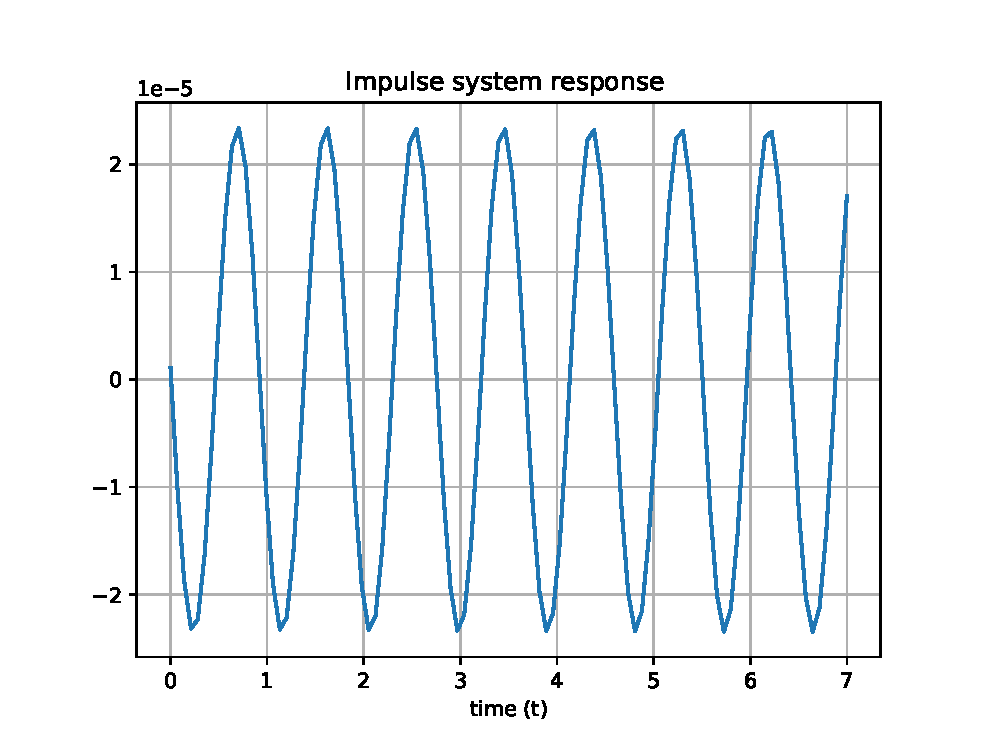
\includegraphics[width=\columnwidth]{./figs/ee18btech11019_5.eps}
\caption{Output when taken from transfer function}
\label{fig:ee18btech11019_plot_1}
\end{figure}
%
The spice simulations are done using the following netlist
\begin{lstlisting}
spice/Draft3.net
\end{lstlisting}
%
and plotted in Fig. \ref{fig:ee18btech11019_plot_2}
%
using the following code.
\begin{lstlisting}
spice/ee18btech11019_2.py
\end{lstlisting}
\begin{figure}[!ht]
\centering
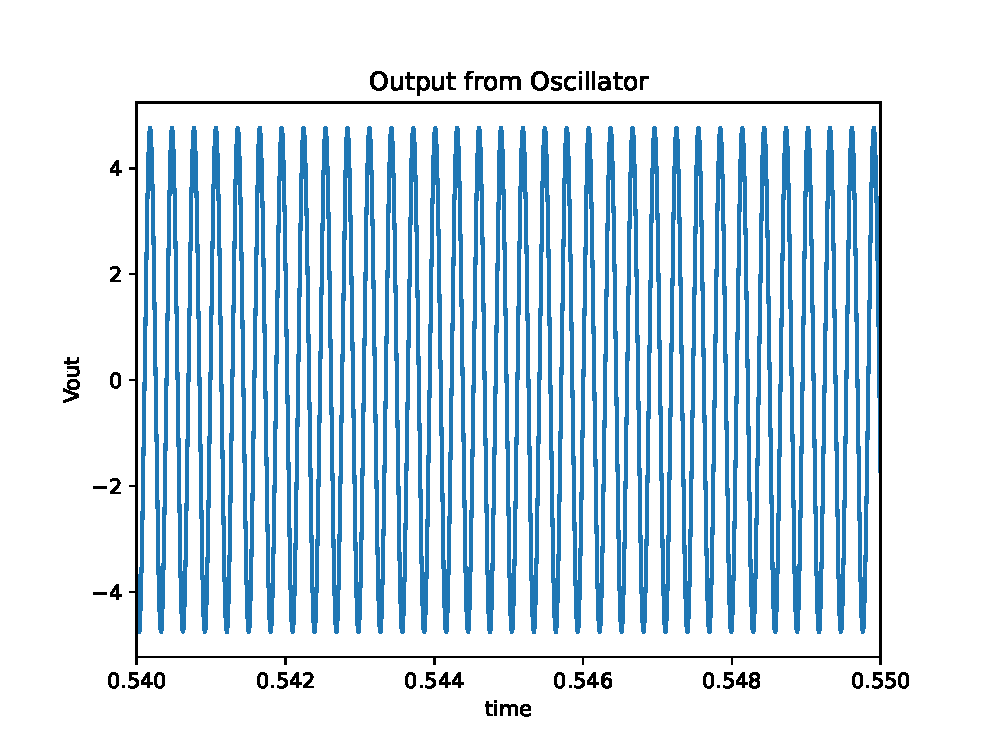
\includegraphics[width=\columnwidth]{./figs/ee18btech11019_6.eps}
\caption{Simulation result}
\label{fig:ee18btech11019_plot_2}
\end{figure}
\renewcommand{\thefigure}{\theenumi}
%
From Fig. \ref{fig:ee18btech11019_plot_2},
the frequency obtained is $3.384$ kHz.  From \ref{eq:ee18btech11019_f}, 
the expected frequency is
\begin{align}
f   &= \frac{1}{2\pi \sqrt{C(L_1 +L_2)}}\\
    &= 3.394 \,kHz
\end{align}
\end{enumerate}
